\documentclass[12pt]{article}
\usepackage{todonotes,setspace,mathtools,microtype,amsfonts,amssymb,graphicx,minted
%,fullpage
}
\title{\vspace{1.5cm}Exploring Patterns in the Divisor Function}
\date{}
\begin{document}
{\hspace{-0.5cm}\includegraphics[width=0.4\textwidth]{../IB.jpg}}
\textbf{\\Glenforest Secondary School\\
Extended Essay}
	{\let\newpage\relax\maketitle}
\vspace{3cm}
\begin{flushright}
\textbf{Candidate Session Number 002203-0031\\
May 2019\\
Mathematics\\
3525 words}
\end{flushright}
\newpage
	\tableofcontents
	\addtocontents{toc}{\textbf{Research Question:} What interesting patterns can be found in the simple divisor function?\\}
	\addtocontents{toc}{\textbf{Thesis:} The divisor function is embedded with patterns such as densities of different values of $\sigma$, minimum starting values of $\sigma$, empty spaces in the log-log interpretation of divisor density, and a link between $\sigma$ and $\pi$. \par}
\newpage
\doublespacing
	\section{Introduction}
		My interest in the divisor function stems from my interest in computing and cryptography. In a highly popular set of cryptographic algorithms known as RSA, prime numbers are extremely important because they only have two divisors (Steyn, 2012). This property, in conjunction with a few others, are the foundations which RSA uses to encode and decode messages and data. Many other cryptosystems also use properties regarding the divisibility of numbers to ensure digital security worldwide.

		With the recent advances in quantum computing, cryptography is coming under scrutiny (Stubbs, 2018). New technologies such as Shor's algorithm are able to harness the power of quantum computers to factor numbers at a significantly faster rate. This means that cryptographic techniques which were once considered unbreakable are now vulnerable to attack as these quantum machines gain computing power. Today, more than ever, it is essential to find new ways to protect our personal data.
		
		As mentioned earlier, properties regarding the divisibility of numbers are the building blocks of modern cryptography. To learn how to better protect our privacy in the quantum age, new patterns of divisibility are explored as they could lead to a more secure form of encryption. As I looked deeper into the fundamentals of RSA, I became interested in number theory, primes, and their properties-- which led me to the divisor function. The divisor function is very simple-- it counts the number of factors/divisors a positive integer has (Weisstein, n.d.). For example, 24 has the divisors 1, 2, 3, 4, 6, 8, 12, and 24; As such, $divisor(24)=8$. In the math community, the divisor function is represented by the Greek letter sigma $(\sigma)$. The formal definition of this function is $\displaystyle\sigma(n)=\sum_{d|n}1$ where $d|n$ means $d$ divides $n$ with no remainder. The divisor function is also sequence A000005 on the On-line Encyclopedia of Integer Sequences.
		
		As I dove deeper into the divisor function, I asked: \textbf{what interesting patterns can be found in the simple divisor function?} This research question is worthy of investigation because 
		of its applications in cryptography, number theory, and algebraic geometry.
		This essay extensively uses the programming language Python and the mathematics package Wolfram Mathematica for numerical analysis and plotting respectively. This essay uses mathematics from fields such as calculus, statistics, set theory, number theory, and more to help answer the research question. Using various analytical techniques, this paper finds patterns among densities of different values of $\sigma$, minimum starting values of $\sigma$, and an unexpected connection between $\sigma$ and $\pi$.
\newpage
	\section{Plotting $\sigma(n)$}
		Various graphs are used to better comprehend information and patterns depending on the type of data. The most common type is the Cartesian coordinate system implemented in the $x$,$y$-plane.
		This is the simple Cartesian plot for the function $\sigma(n)$:
		\begin{figure}[H]
			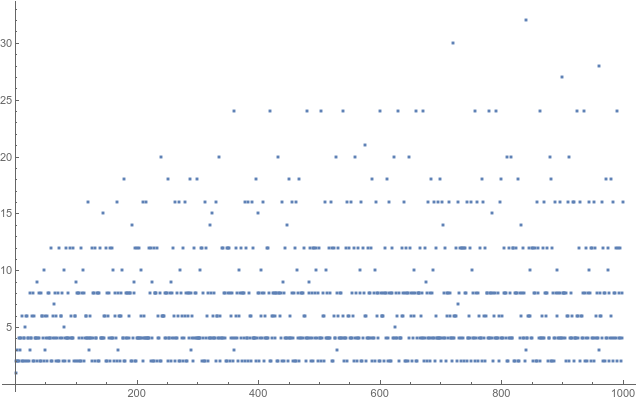
\includegraphics[width=\textwidth]{../Images/nonlogsigma.png}
			\caption{The plot of $\sigma(n)$ for $n\in\{1,2,3,\ldots,1000\}$\label{plainsig}}
		\end{figure}
		This graph shows the discrete nature of the divisor function very well-- the domain and range are the set of positive integers. This limitation forms the distinct horizontal linear patterns (loosely called lines in this essay) created by the aggregation of points. Since the points on a horizontal line have the same $\sigma(n)$ value, they have the same number of divisors. Even though some trends can be seen, $\sigma(n)$ could vary widely between close numbers: making it `chaotic' (Humphrys, n.d.). Due to this chaotic nature, finding more patterns and other interesting properties becomes very difficult, but can patterns come from this chaos? Not much information can be deciphered from this graph; but if a concept of `divisor density' is taken into account, much more might be visible. Divisor density is a different measure of the number of divisors: it measures the ratio of the number of divisors to the number itself: $\dfrac{\sigma(n)}{n}$. For the purposes of this essay, I will use a variant of the Greek letter sigma ($\varsigma$) to represent divisor density $\varsigma(n)=\dfrac{\sigma(n)}{n}$. For example, for $n=24$, $\varsigma(24)=\dfrac{\sigma(24)}{24}=\dfrac{8}{24}=\dfrac{1}{3}$. Divisor density may be a better choice for looking at divisors as it balances the number of factors with the magnitude of the number itself.
		The plot of $\varsigma(n)$ looks like this:
		\begin{figure}[H]
			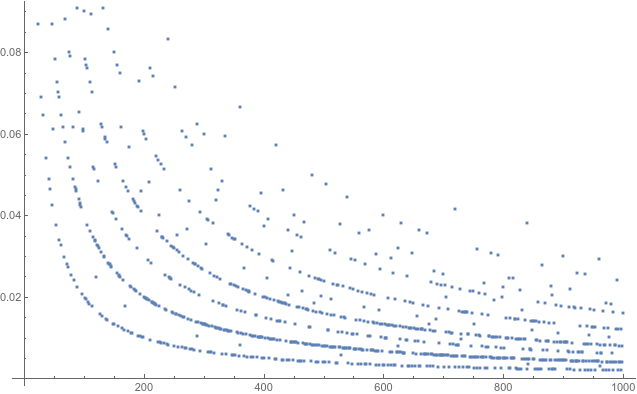
\includegraphics[width=0.8\textwidth]{../Images/varsignonlog.png}
			\caption{The plot of $\varsigma(n)$ for $n\in\{1,2,3,\ldots,1000\}$\label{plainvar}}
		\end{figure}
		Here it is seen that similar to figure~\ref{plainsig}, figure~\ref{plainvar} has patterns of curves instead of lines. In fact, all points from the $\sigma$ function have been transformed as such:
		$$(n,\sigma(n))\to\left( n,\frac{\sigma(n)}{n} \right)$$
		This shows that the points which seem to follow curved lines in figure~\ref{plainvar} actually fall on $\displaystyle{y=\frac{k}{n}}$ for $k\in\mathbb{Z}^+$.

		Here, linearising could help. For functions of the form $y=kx^{-1}$, using a log-log graph reorients the function to show as $\log(y)=\log(k)-\log(x)$ when plotted. Since the mapping shows that $\varsigma$ is of the form $y=kx^{-1}$ (as $y=\varsigma(n)$, $k=\sigma(n)$, and $n=x$), the log-log graph would be useful. This is the function $\varsigma(n)$ plotted on a log-log graph:
		\begin{figure}[H]
			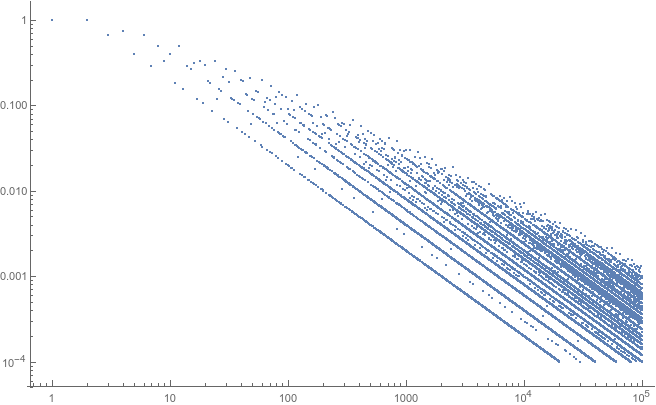
\includegraphics[width=0.9\textwidth]{../Images/plot.png}
			\caption{The plot of $\varsigma(n)$ for $n\in\{1,2,3,\ldots,10^5\}$ on a log-log graph\label{main}}
		\end{figure}
		This is a very useful plot because many patterns can be seen here regarding the distribution of numbers and their divisors. These pattens will be discussed and analysed in Section~\ref{analy}. As I will be exploring patterns in $\varsigma$ through the lens of this plot, it is useful to have more data, so figure~\ref{main} is plotted with $10^5$ data points instead of $10^3$.
	\section{Analysis\label{analy}
		%Divisor Density
		}
		\subsection{The Lines}
			To explain the origination of the downward-sloping lines, lines with a negative gradient, in figure~\ref{main}, the function being plotted $y=\log(\varsigma(\log(n)))$ 
			% (or $y=(\log\circ\,\varsigma\circ\log)(x)$\ )
			must be rearranged to the slope-intercept form of a line.
			Let $y=\log(\varsigma(x))$ and $x=\log(n)$ as determined by the use of the log-log graph.
			\begin{align*}
				\varsigma(n)&=\frac{\sigma(n)}{n}\\
				\log(\varsigma(n))&=\log(\sigma(n))-\log n\\
				y&=\log(\sigma(n))-x\\
				y&=-x+\log(\sigma(n))
			\end{align*}
			Comparing $y=-x+\log(\sigma(n))$ with the standard form $y=mx+b$, it is seen that $m=-1$, and $b=\log(\sigma(n))$.

			This result explains that each of the lines have a slope (i.e.\,gradient) of $-1$ and start at a height of $\log(\sigma(n))$.

			The slope of $-1$ does not come from some property of the factors, but instead the definition of divisor density. Since $\varsigma(n)=\dfrac{\sigma(n)}{n}$, the $-1$ comes from the dividing by $n$ operation. If $\varsigma$ was defined as $\dfrac{\sigma(n)}{n^k}$ instead for any constant $k$, then the slope would be $-k$. As such, the slope in this respect does not convey any relevant information about the nature of the divisor function, and is just an artefact of the definition.

			Since all lines share the same slope, the only remaining differentiating factor is their $y$-intercept: $b=\log(\sigma(n))$. If two lines are not coincident, but share the same slope, they must be parallel and have different $y$-intercepts. Since $b=\log(\sigma(n))$, the $y$-intercept is determined by the number of factors the points in that line have. Thus, different lines have different results for $\sigma(n)$. Additionally, it is concluded that each set of points on a line share a common number of divisors. The lowest line would have the lowest number of divisors since it would minimize $b=\log(\sigma(n))$ by minimizing $\sigma(n)$. The set of numbers with the least factors are the prime numbers (excluding $\sigma(1)=1$) as they minimize $\sigma$ with $\sigma(n)=2$. As such, the y-intercept of the lowest line is $b=\log(2)$. As the number of divisors increases, the height of the line increases.

			The interesting piece here is that in figure~\ref{main}, the lines get more dense as $\varsigma$ and $n$ increase. The explanation is that $\log(x)$ is an increasing function at a decreasing rate (i.e.\,$\dfrac{\mathrm{d}\log(x)}{\mathrm{d}x}>0 \text{ and } \dfrac{\mathrm{d}^2\log(x)}{\mathrm{d}x^2}<0$ for all $x>0$). This means that even though a line with numbers which have more divisors is higher, it won't be spaced out as much-- which makes it seem more densely packed.
		\subsection{The Number of Points in a Line}
			\begin{figure}[H]
				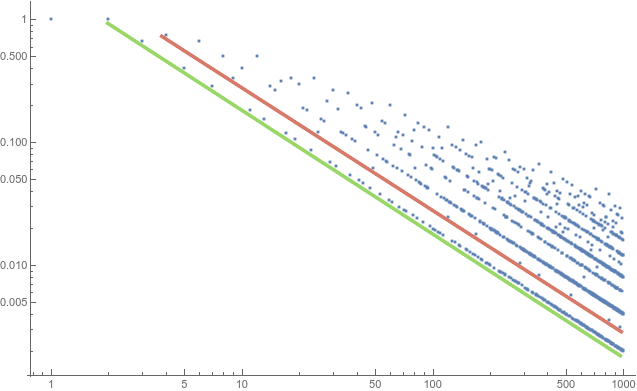
\includegraphics[width=\textwidth]{../Images/HLPlot.png}
				\caption{The plot of $\varsigma(n)$ for $n\in\{1,2,3,\ldots,1000\}$ with $\sigma(n)=2$ and $\sigma(n)=3$ underlined\label{HLPlot}}
			\end{figure}
			Compare the linear pattern representing $\sigma(n)=2$ (underlined with green in figure~\ref{HLPlot}) and $\sigma(n)=3$ (underlined with red in figure~\ref{HLPlot}). The prime-number pattern has significantly more points than the pattern with 3 divisors. Why?

			First off, what allows a number to have 3 factors?
			Usually numbers have an even number of factors as $ab=c$ means $a$ and $b$ are factors of $c$ (given $a\in\mathbb{Z^+}$ and $b\in\mathbb{Z^+}$). A possible method to count to number of factors is to repeat the process above an appropriate number of times and check how many distinct factors are found. Each time the $ab=c$ process is confirmed, 2 new factors are found- unless $a=b$. This means that $c$ can be written as $a^2$- meaning that $c$ is a perfect square. The conclusion here is that if $\sigma(c)$ is odd, $c$ is a perfect square.

			For a number to have 3 factors, it needs to be a square of a prime. To demonstrate, I'll use a proof by contradiction using Euclid's Lemma (S\'eroul, 2000). Suppose $p$ is prime. If on the contrary there exists another number $n\in\mathbb{Z}^+$ such that it divides the square of the prime (i.e.\ $n$ divides $p^2$ with no remainder) and $n$ is not $1$, $p$, or $p^2$. Euclid's Lemma states that ``if $n$ divides $ab$, and $n$ is relatively prime to $a$, then $n$ divides $b$''. Since $p$ is prime, $n$ is coprime to it. Applying the lemma with $a=p$ and $b=p$ implies that $n$ divides $p$; contradicting that it is different from either 1 or $p$, thus proven.

			For a number to have 3 factors, it has to be a square of a prime. Now the question remains, why does the line representing $\sigma(n)=3$ have so few points?
			As $\sigma(n)=2\iff \sigma(n^2)=3$, and $\displaystyle{x>1\implies \frac{\text{d}\,x^2}{\text{d}\,x}>1}$, the `squaring' transformation in $\sigma(n^2)$ takes the input and `spreads out' the output. That is to say, for all $a,b>1$ and $a\neq b$, the distance between $a$ and $b$ is less than the distance between $a^2$ and $b^2$ (i.e.\,$|a-b|<|a^2-b^2|$). This spreading mechanism is the reason why $\sigma(n)=3$ is relatively sparse.

			This means that in a range $[1,k]$, for integer $k\geq 2$, the amount of numbers with 2 factors will be more than the amount of numbers with 3 factors. For example, $n\in\{2,3,5\}$ for $\sigma(n)=2$ maps to $n\in\{4,9,25\}$ for $\sigma(n)=3$.

			In addition to $\sigma(n)=3$, it can be seen that the lines corresponding to odd factors are all less populated than the lines corresponding to even factors. As previously mentioned, odd factors implies the number is a perfect square. The concept that squaring `spreads' a distribution, can be applied here again, to show why the lines corresponding to odd factors are less dense than the lines of even factors. Since there are unlimited examples of $n$ for both $\sigma(n)=2$ and $\sigma(n)=3$, the density of the lines needs to be considered instead of the total amount. Here, density means that in the set of positive integers $[1,k]$ for any integer $k\geq 2$, there are more instances of $\sigma(n)=2$ than $\sigma(n)=3$.
			%$$\forall( k\in\mathbb{Z}^+\land k\geq 2\land(\sigma(n)=2\lor\sigma(n)=3)): \sum_{n=1}^k2\times(\sigma(n)-2.5)<0$$
		\subsection{Starting Points of Lines\label{TPRsec}}
			Looking at figure~\ref{main}, as the $\sigma$ value of the lines increases (corresponding to the height of the line), they start at a higher $n$ value. What causes this phenomenon?

			I wrote some code to isolate the start of each line (Appendix~\ref{TopRowCode}) by isolating the first number to reach a new number of factors (for example, 192 is the first number to have 12 factors). Plotting the $\varsigma$ values for these on a log-log plot resulted in the following:
			\begin{figure}[H]
				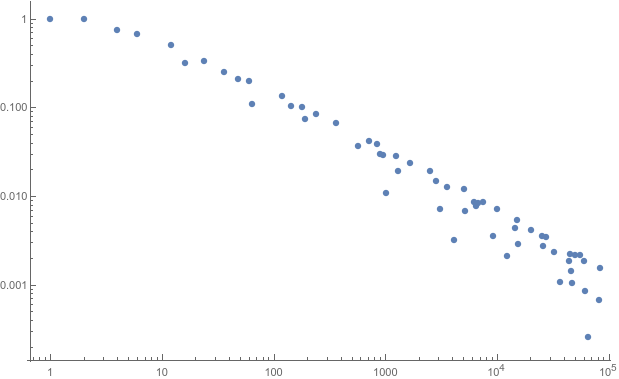
\includegraphics[width=1.0\textwidth]{../Images/toprow.png}
				\caption{The plot of $\varsigma(n)$ on a log-log graph for the first values of $n<10^5$ which have a new number of factors
				%\footnote{$n\in\{1,2,3\ldots,10^5\} \cup\{k|k\in\mathbb{Z}^+,\nexist w\in\mathbb{Z}^+,w<k:\sigma(w)=\sigma(k)\}$}
				\label{TRP}}
			\end{figure}
			Here, it is clear that there is a pattern regarding where a line starts. As seen in figure~\ref{plainsig}, the $\sigma$ function is chaotic, so there is no effective approximation in elementary functions for $\sigma(n)$. Since there is no approximation for $\sigma(n)$ in elementary functions, there is no algebraic manipulation of an elementary function derived from $\sigma(n)$ which be used to find a pattern in figure~\ref{TRP}.

			One method to count the number of divisors of $n$ is to count the number of factors less than or equal to $\sqrt{n}$, double that amount, and finally subtract 1 if $n$ is a perfect square. This technique comes from the realization that half of all factors of $n$ are less than $\sqrt{n}$ since the largest possible value of the low factor pairs ($a$ in $a\leq b$ such that $ab=n$) is $\sqrt{n}$. Using this method, it can be assumed that a very rough upper bound could be $\sigma(n)< 2\sqrt{n}$. Using this approximation, $\varsigma(n)<\dfrac{2\sqrt{n}}{n}= 2n^{-\frac{1}{2}}$. Plotting this result shows:
			\begin{figure}[H]
				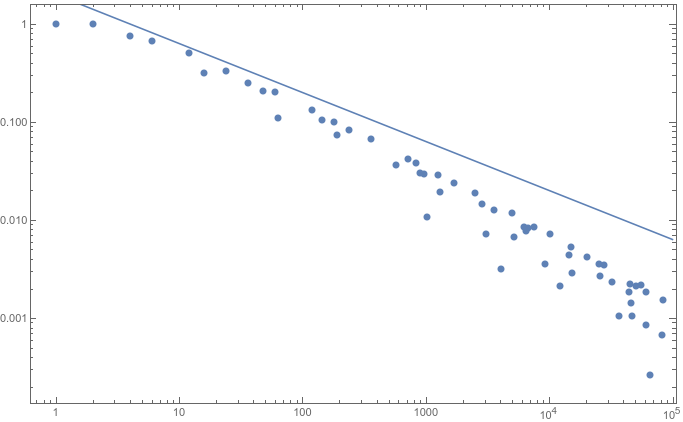
\includegraphics[width=\textwidth]{../Images/TRPsqrtREG.png}
				\caption{The $\varsigma(n)< 2n^{-\frac{1}{2}}$ regression overlapped on figure~\ref{TRP}\label{TRPsqrt}}
			\end{figure}
			\vspace{-0.5cm}
			Looking at the axes of this graph, notice that the refrence numbers increase exponentially (e.g.\ 10 to 100 to 1\,000). This applies both to the $x$ and $y$ axis. The effect of this change is that power functions are represented as linear on this graph. This can directly be seen in the function $y=2n^{\frac{-1}{2}}$ and how it seems linear.

			The upper bound of $\varsigma(n)< 2n^{-\frac{1}{2}}$ is close for small values of $n$, but quickly worsens for larger values of $\varsigma$. When taking into consideration that this is a log-log plot, the approximation seems worse-- for example, near $n\approx 10^5$, $\varsigma$ and $2n^{\frac{-1}{2}}$ differ by almost a factor of 5.

			Simply looking at figure~\ref{TRPsqrt} shows the problem: a wrong slope. 
			\begin{align*}
				y&=ax^k\\
				\log y&=\log a+k\log x\\
				\log y&=k\log x+\log a
			\end{align*}
			The equations above show that the slope of the line is controlled by the exponent, and the $y$-intercept is controlled by the coefficient of $x^k$. Correcting for the fact that this is a log-log plot, this means that the approximation has the wrong exponent. Decreasing the exponent would decrease the slope. 
			Simply by numerically manipulating the variables $a$ and $k$, I found that $\varsigma(n)< 3.2n^{-\frac{2}{3}}$ works well:
			\begin{figure}[H]
				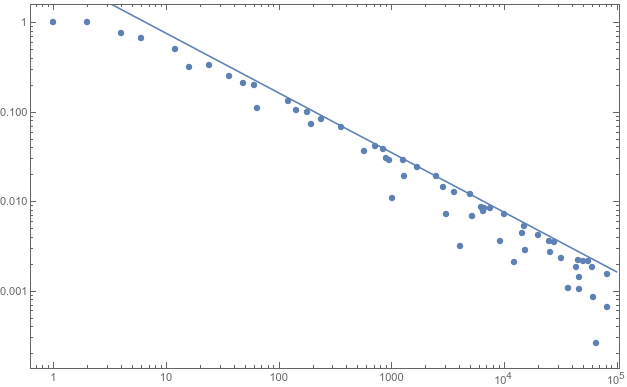
\includegraphics[width=0.7\textwidth]{../Images/GoodReg.png}
				\caption{The $\varsigma(n)< 3.2n^{-\frac{2}{3}}$ regression overlapped on figure~\ref{TRP}\label{TRPgood}}
			\end{figure}
			This upper bound is significantly better than the previous, and the following graphic comparing the bounds $3.2n^{-\frac{2}{3}}$ and $2\sqrt{x}$ with $\varsigma$ is effective in showcasing the drastic improvement:
			\begin{figure}[H]
				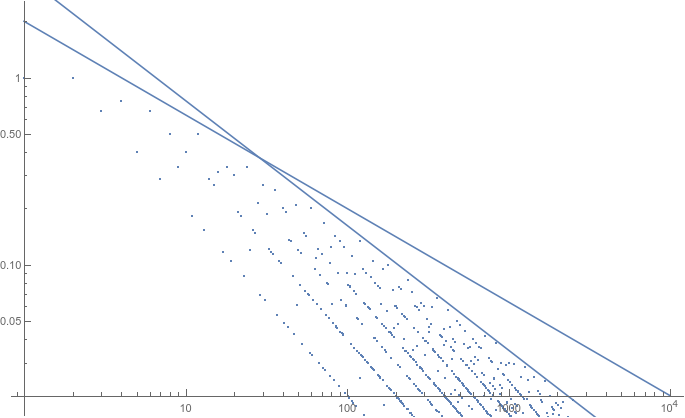
\includegraphics[width=1.0\textwidth]{../Images/RegComp.png}
				\caption{The upper bounds of $\varsigma(n)< 3.2n^{-\frac{2}{3}}$ and $\varsigma(n)< 2n^{-\frac{1}{2}}$ being compared\label{TRPcomp}}
			\end{figure}
			The two bounds intersect at $n\approx 28.7$, showing that the new upper bound is better for $n\geq 29$. Again, note that the ``3.2'' constant was found using visual approximation (i.e.\ manipulating the coefficient until it `looked close'). A better method for computing this constant will be explored later in this essay.
			%Why is this new upper-bound worse for numbers less than 29? The answer lies in a statistical concept known as the law of large numbers\todo[fancyline]{cite}. The law of large number
		\subsection{The Empty Spaces}
			Going back to figure~\ref{main}, there are two spaces which don't have points: the bottom left, and the top right.
			\subsubsection{The Bottom Left}
				As proven earlier, the lowest line constitute the prime numbers, which follow the line $\log y=-\log x+\log 2$. Since primes have the fewest number of factors (excluding $n=1$), they act as a limiting line for divisor density. Since no number can have any fewer factors, there are no points seen in the bottom left of figure~\ref{main}. This is with the exclusion of $n=1$ which has only 1 factor. This point can be seen to the right of the prime number line as expected, but since it is only 1 point, it is ignored for much of this essay.
			\subsubsection{The Top Right}
				Opposite to the other empty space, the top right of figure~\ref{main} is also empty. Explaining this area is more tricky as there is no clear separating entity (unlike the primes for the bottom left). As stated in Section~\ref{TPRsec}, $\varsigma(n)< 3.2n^{-\frac{2}{3}}$, so the empty space is the area represented by $y> 3.2x^{-\frac{2}{3}}$, or accounting for the log-log graph, $\log y> \log(3.2)-\dfrac{2x}{3}$.
				
				Even though this may seem like a tempting conclusion, the result $\log y> \log(3.2)-\dfrac{2x}{3}$ provides information with no understanding of the reason. Why is this inequality preventing $\varsigma(n)$ from going any higher?

				Maybe going back to the basics might help: finding what this upper bound says about the standard divisor function.
				\begin{align*}
					\varsigma(n)&< 3.2n^{-\frac{2}{3}}\\
					\frac{\sigma(n)}{n}&< 3.2n^{-\frac{2}{3}}\\
					\sigma(n)&< 3.2n^{\frac{1}{3}}\\
					\sigma(n)&< 3.2\sqrt[3]{n}\\
					\max_{k\in\{1,2\ldots,n\}}\sigma(k)&\propto \sqrt[3]{n}
				\end{align*}
				The proportionality constant (constant multiplied with $\sqrt[3]{n}$ to create the most efficient upper bound for $\sigma$) of 3.2 was found by visual approximation, and it may change as better methods to estimate it are found, but, in figure~\ref{TRPgood}, it was very clear that the slope was $\dfrac{-2}{3}$ and that value was found to be very accurate and precise. As such it can be said that $\max\limits_{k\in\{1,2\ldots,n\}}\sigma(k)\propto \sqrt[3]{n}$. What this means that the maximum of the $\sigma$ function for integer arguments between 1 and $n$ (inclusive) is proportional to $\sqrt[3]{n}$. As seen if figure~\ref{plainsig}, the $\sigma$ function is chaotic, but its top boundary was well defined. To represent this boundary, the $\max$ operator from set theory was used. The switch from $<$ to $\propto$ is important as proportionality allows for describing the function in a more general way-- allowing for other estimations of the coefficient.
				
%				Plotting $\sigma(n)$ and $3.2\sqrt[3]{n}$ better displays the clear boundary:
%				\begin{figure}[H]
%					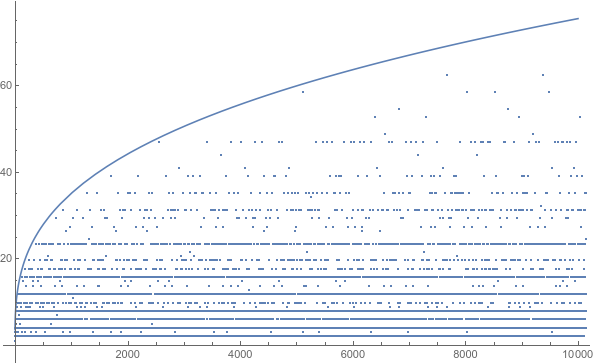
\includegraphics[width=\textwidth]{../Images/sigreg.png}
%					\caption{$\sigma(n)$ and $3.2\sqrt[3]{n}$ graphed on a Cartesian plot\label{SigReg}}
%				\end{figure}
			\subsection{Computing the Proportionality Constant}
				Let the proportionality constant (coefficient of $\sqrt[3]{n}$) be $w$.
				\begin{align*}
					\sqrt[3]{n}&\propto \max_{k\in\{1,2\ldots,n\}}\sigma(k)\\
					w\sqrt[3]{n}&\approx \max_{k\in\{1,2\ldots,n\}}\sigma(k)\\
					w&\approx \frac{\max\limits_{k\in\{1,2\ldots,n\}}\sigma(k)}{\sqrt[3]{n}}\\
					w&=\lim_{j\to\infty}\frac{\sum\limits_{n=1}^{j}\frac{\max\limits_{k\in\{1,2\ldots,n\}}\sigma(k)}{\sqrt[3]{n}}}{j}
				\end{align*}
				In the steps above, $w$ is isolated. In the last step, $w$ is no longer approximate, and is defined as the average expected value of $w$ among all positive integers.

				Trying an example with $n=1000$, $\sigma(n)$ for $k\leq1000$ is maximized at $k=840$ with $\sigma(840)=32$
				\begin{align*}
					w&\approx \frac{\max\limits_{k\in\{1,2\ldots,n\}}\sigma(k)}{\sqrt[3]{n}}\\
					w&\approx \frac{32}{\sqrt[3]{840}}\\
					w&\approx \frac{16}{105}\sqrt[3]{11025}\\
					w&\approx 3.39
				\end{align*}

				\vspace{-0.4cm}Using python code (Appendix~\ref{coProp}), the predicted values for $w$ (using the averaging method) were found for all positive integer $j\leq 10\,000$ in an attempt to look for convergence:
				\begin{figure}[H]
					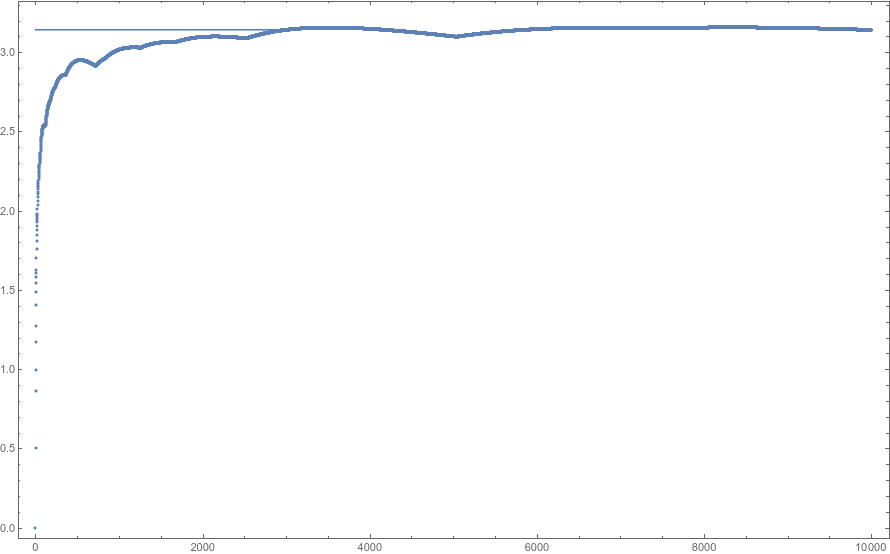
\includegraphics[width=1\textwidth]{../Images/SupPi.png}
					\caption{Predicted values for $w$ with $j\in\{1,2,3,\ldots,10\,000\}$ and a horizontal line at $y=\pi$\label{pi}}
				\end{figure}
				As seen computationally, $w$ approaches $\pi$. So, $\pi\sqrt[3]{n}\approx \max\limits_{k\in\{1,2\ldots,n\}}\sigma(k)$. This also means that in terms of divisor density, $\varsigma(n)\lesssim \pi\sqrt[3]{n}$. ``$\lesssim$'' is the symbol for approximately less than.

				Here, unlike other graphs, 10\,000 points were used. This is because of computational limitations: I left my computer running overnight to gather as many data points as possible, and I had just over 10\,000 values. Even though this is less than the typical 100\,000 points in the rest of this paper, it provides enough evidence to support the connection between $\sigma$ and $\pi$.
\newpage
				Use of the symbol $\lesssim$ in $\varsigma(n)\lesssim \pi\sqrt[3]{n}$ is intentional. To explain this, note that in figure~\ref{pi} the initial estimate (i.e.\, low $j$ value) for $w$ is poor and then it quickly converges to $\pi$. If $w$ is set to $\pi$, and the $\sigma(n)\lesssim\pi\sqrt[3]{n}$ upper-bound is checked for small values of $n$, it would seem incorrect. For example, using figure~\ref{pi}, the best estimate for $w$ for $n<500$ would be $w=3$ instead of $w=\pi$. This means that $w=\pi$ is useful for the $\sigma$ (or $\varsigma$) function as a whole, or large values/ranges of those functions but not necessarily for a small set of numbers or a set of small numbers.

				The fact that this limit converges provides additional evidence that the estimate that $\max\limits_{k\in\{1,2\ldots,n\}}\sigma(k)\propto \sqrt[3]{n}$ as having an incorrect exponent would result in a divergent sequence.

				At this point, definitively proving the result of $w=\pi$ is excessive for the extended essay and may also be too difficult to prove in such a short period of time. Due to these restrictions, I have instead opted to turn the result into the following conjecture:
				$$\lim_{j\to\infty}\frac{\pi\sqrt[3]{j}}{\max\limits_{n\in\{1,2,3,\ldots,j\}}\sigma(n)}=1$$

				Another interesting observation in figure~\ref{pi} which is excessive for this essay is the `bouncing' pattern in the convergence sequence (i.e.\ the estimates for $w$ seems to quickly approach, and then slowly move away from $w=\pi$ repeatedly)
	\newpage
	\section{Conclusion}
		In this essay I explored many patterns which could be found in the divisor function such as densities of different values of $\sigma$, minimum starting values of $\sigma$, empty spaces in the log-log interpretation of divisor density, and a link between $\sigma$ and $\pi$. These patterns answer my research question: what interesting patterns can be found in the simple divisor function? To be able to find any of these patterns, I had to call upon my knowledge from various fields of mathematics: number-theory, set-theory, algebra, and calculus. It really surprised me how much these seemingly separate fields are connected. For example, when I was trying to understand why numbers with an odd number of factors were uncommon, I had to use number and set theory to figure out they are perfect squares; then use calculus to understand the spreading effect; and finally algebraically manipulate my solution. At school I learnt that calculus was a study of change-- smooth change; and here I was applying it to the exact opposite: a discrete chaotic function. I find that this exploration of mathematics has pushed me to become mathematically creative to an extent I never have been before. The level of hidden information and patterns in a simple function continued to surprise me from start to finish.

		 %When I started, it was difficult to find patterns because of how to data was presented: in a simple Cartesian graph. As I progressed, I transformed the function in various way to make it easier to work with: using a log-log plot, isolating points, creating a whole new function, and more. I realized the value of modifying something common into something familiar. Next, I used my new creations to find patterns such as the lines, point density, and empty spaces. But, before I could try to find these patterns I had to call upon my knowledge from various fields of mathematics: number-theory, set-theory, algebra, and calculus. It really surprised me how much these seemingly separate fields are connected. For example, when I was trying to understand why numbers with an odd number of factors were uncommon, I had to use number and set theory to figure out they are perfect squares; then use calculus to understand the spreading effect; and finally algebraically manipulate my solution. At school I learnt that calculus was a study of change- smooth change; and here I was applying it to the exact opposite: a discrete chaotic function. In the beginning I asked ``What patterns can be found in the divisor function?''. Throughout this essay, novel patterns were found such as the distribution of divisors, the rate of growth for $\sigma(n)$, and empty spaces. There still is an additional question: what is the significance of the proportionality constant $\pi$ This question has arisen as a result of my research and I do not yet have an answer. This question could not be addressed in this essay due to limitations in time, as well as my mathematical ability.

%		As I approached the end, I was feeling proud of my accomplishment but felt a lack regarding how much the world would care about it. The value of a discovery is determined by its applications. What are the applications of this work? The divisor function shows up in the study of modular forms and elliptic curves, which makes it significant in algebraic geometry and in cryptography. And that's it. That's when I realized that this is the nature of mathematics research. Mathematical research is not intended for the present, but rather for the future. Conic sections were studied as pure math in ancient Greece, and were applied 2000 years later in Newtonian physics to describe planetary orbits.
%
%		Mathematics is beautiful to most people because of how well it serves itself as a tool to solve real-world problems. Mathematics is beautiful to me and many other mathematicians because of other reasons. To us, math it is a construction of the human imagination- governed my the simplest of rules (axioms)- and the emergent properties are abundant with their own complex universe of unexpected patterns and processes. Simply counting the number factors can lead to an entire essay.\todo[fancyline]{paragraph discouraged as per EE report}

\newpage
\singlespacing
	\section{Appendix}
			\subsection{Divisor Function\label{divfun}}
				\begin{minted}{python}
def sigma(num):
	"""
	returns the number or factors for a positive integer n
	"""
	nfactors = 0 # the number of factors of n
	for divisor in range(1, num+1): # divisors: {1,2,3,4..,n}
		if num%divisor == 0: # divides with no remainder
			nfactors += 1 # i.e one new factor found
	return nfactors
				\end{minted}
			\subsection{All Data}
				\begin{minted}{python}
"""
outputs factor data for all numbers up to specified amount
to the `alldata' file
"""
from functions import sigma, filewrite

max_num = int(raw_input("How many data points do you want?\n"))
data = '{' # to conform to Mathematica format															 '{'
for current_number in range(1, max_num): # current_number is {1,2,3..,to-1}
    # appending appropriate ratio to data
    data += str(sigma(current_number)/float(current_number)) + ', '
data += str(sigma(max_num)/float(max_num)) + '}' # last point: to; "}"
					         # to conform to Mathematica
filewrite('alldata', data)
				\end{minted}
			\subsection{Top Row\label{TopRowCode}}
				\begin{minted}{python}
"""
finds toprow points and outputs to `toprow' file
"""
from functions import filewrite, sigma
# first; sigma; filewrite

TOP = int(raw_input("How many toprow points do you want to go through?\n"))
faclst = map(sigma, range(1, TOP+1))
found = []
nfl = [] # in the format [number, ratio]
for r in range(len(faclst)):
    i=[r,faclst[r]]
    if i[1] not in found:
        found.append(i[1])
        nfl.append([i[0]+1, float(i[1])/(i[0]+1)])
del faclst
del found
out = '{'
for i in nfl:
    out += '{'+str(i[0])+','+str(i[1])+'},'
out = out[0:len(out)-1]
out += '}'
filewrite('toprow', out)
				\end{minted}
			\subsection{Finding the Proportionality Constant\label{coProp}}
				\begin{minted}{python}
from functions import sigma, filewrite
compare_to=int(raw_input("Till what n value to compare to?\n"))
output="{"
for limit in range(1,compare_to+1):
    data_set=[]
    max_sigma=-1
    for n in range(1,limit):
        divs=sigma(n)
        if divs>max_sigma:
            max_sigma=divs
        data_set.append(1/((float(i)**(1/3.))/max_sigma))
    output+='{'+str(limit)+','+str(sum(data_set)/limit)+'},'
    print limit*1./compare_to
output=output[0:-1]
output+='}'
filewrite("testfile",output)
				\end{minted}
\newpage
	\section{References}
		\texttt{\ \ \ \ \ \ \ \ \ \ \ \ \ \ \ \ \ \ \ \ \ \ \ \ \ \ \ \ \ \ \ \ \ \ \ \ \ \ \ \ \ \ \ \ \ \ \ \ \ \ \ \ \ \ \ \ \ \ \ \ \ \ \ \ \ \ \ \ \ \ \ \ \ \ \ \ \ \ \ \ \ \ \ \ \ \ \ \ \ \ \ \ \ \ \ \ \ \ \ \ \ -}

		Humphrys, M. (n.d.). Chaotic functions. Retrieved September 4, 2018, from http://computing.dcu.ie/$\sim$humphrys/Notes/Neural/chaos.html

		\vspace{1cm}

		S\'eroul, R. (2000). Programming for mathematicians. Berlin: Springer.

		\vspace{1cm}

		Steyn, B. (2012, May 26). How RSA Works With Examples. Retrieved September 4, 2018, from http://doctrina.org/How-RSA-Works-With-Examples.html

		\vspace{1cm}

		Weisstein, E. W. (n.d.). Divisor Function. Retrieved from \\http://mathworld.wolfram.com/DivisorFunction.html

		\vspace{1cm}

		Stubbs, R. (2018, April 29). Quantum Computing and its Impact on Cryptography. Retrieved from https://www.cryptomathic.com/news-events/blog/quantum-computing-and-its-impact-on-cryptography
\end{document}
